\documentclass{article}

\usepackage{neurips_2025}
\workshoptitle{Lock-LLM}

\usepackage[utf8]{inputenc}
\usepackage[T1]{fontenc}
\usepackage{hyperref}
\usepackage{url}
\usepackage{booktabs}
\usepackage{amsfonts}
\usepackage{nicefrac}
\usepackage{microtype}
\usepackage{xcolor}
\usepackage{amsmath}
\usepackage{graphicx}

\title{CLSA: Cross-Lingual Summarization as a Black-Box Watermark Removal Attack}

\author{Gokul Ganesan \\
  Department of Computer Science\\
  New York University\\
  New York, NY 10003 \\
  \texttt{gokul@nyu.edu, gokulganesan3@gmail.com} \\
}

\begin{document}

\maketitle

\begin{abstract}
Watermarking has been proposed as a lightweight mechanism to identify AI-generated text, with schemes typically relying on perturbations to token distributions. While prior work shows that paraphrasing can weaken such signals, these attacks remain partially detectable or degrade text quality. We demonstrate that cross-lingual summarization attacks (CLSA) — translation to a pivot language followed by summarization and optional back-translation — constitutes a qualitatively stronger attack vector. By forcing a semantic bottleneck across languages, CLSA systematically destroys token-level statistical biases while preserving semantic fidelity. In experiments across multiple watermarking schemes (KGW, SIR, XSIR, Unigram) and five languages (Amharic, Chinese, Hindi, Spanish, Swahili), we show that CLSA reduces watermark detection accuracy more effectively than monolingual paraphrase at similar quality levels. Our results highlight an underexplored vulnerability that challenges the practicality of watermarking for provenance or regulation. We argue that robust provenance solutions must move beyond distributional watermarking and incorporate cryptographic or model-attestation approaches. On 300 held-out samples per language, CLSA consistently drives detection toward chance while preserving task utility, and it outperforms back-translation in most settings. Concretely for \textbf{XSIR} (explicitly designed for cross-lingual robustness), AUROC with paraphrasing is $0.827$, with Cross-Lingual Watermark Removal Attacks (CWRA)~\citep{He2024cwra} using \emph{Chinese} as the pivot it is $0.823$, whereas CLSA drives it down to $0.53$ (near chance). Results highlight a practical, low-cost removal pathway that crosses languages and compresses content without visible artifacts.
\end{abstract}

\section{Introduction}

Text watermarking aims to embed provenance signals in generative outputs by slightly biasing token sampling. In practice, these signals must survive downstream editing, translation, and summarization if they are to support provenance or policy enforcement in realistic workflows. Prior work has shown that monolingual paraphrasing or back-translation can weaken detectors, but the effect is uneven and often trades off with utility. We study a more damaging and practical transformation: a Cross-Lingual Summarization Attack (CLSA) that first translates a watermarked passage into a pivot language, then compresses it with abstractive summarization, optionally followed by back-translation to the original language. This pipeline forces a semantic bottleneck and alters subword structure and length statistics in ways that jointly target the cues exploited by modern detectors.

Our evaluation combines four representative detectors—KGW, SIR, XSIR, and Unigram—with five languages spanning diverse morphology and scripts (Amharic, Chinese, Hindi, Swahili, Spanish). Using public translation and summarization models (M2M100 and mT5/XLSum), we compare CLSA against back-translation, monolingual paraphrasing, and cross-lingual rewriting without summarization (CWRA)~\citep{He2024cwra} on held-out sets (300 test and 200 validation samples per language). Across detectors and languages, CLSA consistently drives detection toward chance while maintaining short, readable outputs. For example, representative AUROCs for CLSA cluster around 0.5 for XSIR on Amharic (~0.49), Chinese (~0.54), and Spanish (~0.51), and remain low for KGW on Spanish (~0.58), whereas back-translation and paraphrasing often leave stronger residual signals (e.g., Unigram on Hindi ~0.61 under back-translation). In addition, TPR at 1% FPR is typically near zero under CLSA, indicating detectors struggle to operate at low false-positive rates.

Why does CLSA work better than simpler transformations? Summarization removes many seeded positions and collapses multiple paraphrastic realizations into a shorter form, disrupting local n-gram and position-dependent patterns. Cross-lingual translation perturbs tokenization boundaries and vocabulary support, further diluting distributional biases. Empirically, we observe higher EER and lower Accuracy@thr and F1@thr for CLSA than for back-translation or paraphrase at comparable utility levels, suggesting the combination of cross-lingual rewriting and length compression is the key lever rather than either component alone.

From a deployment standpoint, the attack is black-box and low-cost. It requires no access to watermark keys or detector internals, relies only on commodity models, and yields outputs that remain useful for common downstream tasks. This raises a concrete risk for watermark-based provenance: adversaries can remove signals without heavy optimization or bespoke training, and they can do so across languages where detectors may already be brittle.

We position our contributions as follows:
\begin{enumerate}
    \item \textbf{Attack formulation:} We define CLSA and provide a simple black-box pipeline using public translation and summarization models.
    \item \textbf{Multi-language, multi-detector study:} We evaluate KGW, SIR, XSIR, and Unigram across Amharic, Chinese, Hindi, Swahili, and Spanish, and benchmark against back-translation, paraphrasing, and CWRA~\citep{He2024cwra}.
    \item \textbf{Mechanistic analysis:} We explain why summarization plus cross-lingual transfer suppresses seeded-token bias, n-gram locality, and support overlap more than translation alone.
    \item \textbf{Implications and defenses:} We discuss length-aware detectors and semantic-clustered watermarking as partial mitigations, and argue for augmenting distributional watermarks with cryptographic or attestation-based provenance signals.
\end{enumerate}

Taken together, our findings indicate that cross-lingual summarization is a practical removal pathway that current watermark detectors do not reliably withstand. As LLM outputs circulate through translation and summarization tools, provenance mechanisms will need to anticipate and defend against this compound transformation or risk frequent failure in the wild.

\section{Related Work}

\textbf{Distributional watermarking for LLMs.}
Early methods embed provenance signals by perturbing token probabilities during generation.
The keyed-green-list (KGW) scheme of \citet{kirchenbauer2023watermark} introduced a hash-seeded partition of the vocabulary, biasing "green" tokens upward so that watermarked text contains an abnormally high fraction of them.
Subsequent work explored unbiased logit shifts, entropy-aware detection, and public-key variants, but all inherit KGW's reliance on token-level frequency cues and thus struggle when those cues are disrupted.

\textbf{Cross-lingual watermark removal attacks.}
Most robustness studies focus on monolingual paraphrasing or copy-paste noise; cross-lingual transformations remained underexplored until the Cross-Lingual Watermark Removal Attack (CWRA)~\citep{He2024cwra}.
CWRA wraps the user's prompt in a pivot language, obtains the LLM's answer in that language, and finally translates the response back, effectively erasing distributional traces while preserving semantics.
Empirically, CWRA drives detector AUROC close to random while maintaining high ROUGE quality, outperforming back-translation and paraphrase baselines.
Its simplicity—and the fact that it requires only off-the-shelf MT systems—highlights a practical threat to watermarking in multilingual settings.

\textbf{Semantic-invariant and cross-lingual defenses.}
To counter rewriting attacks, \citet{liu2024sir} proposed the Semantic Invariant Robust (SIR) watermark, which assigns correlated logit shifts to semantically similar prefixes so that paraphrases share the same watermark signature.
While SIR improves resilience to monolingual paraphrasing, its cross-lingual consistency is still limited; the CWRA paper shows that SIR's AUROC can fall below 0.7 after a translate–translate-back cycle.
Follow-up work (X-SIR) clusters tokens across languages before biasing them, partially restoring detectability but at the cost of added model-specific training.
Our CLSA attack builds on this line, demonstrating that an additional \emph{summarization} bottleneck collapses seeded positions and vocabulary overlap, yielding even lower detection accuracy than CWRA.

\section{CLSA: Cross-Lingual Summarization Attack}

\textbf{Novelty and intuition.}
CLSA is a \emph{translate $\rightarrow$ compress $\rightarrow$ (optional) back-translate} pipeline designed to erase distributional watermarks by forcing information through a \emph{semantic bottleneck}. Unlike CWRA—which (i) \emph{prompts the LLM in a pivot language} $\ell_p$ and (ii) performs translate $\rightarrow$ retranslate without compression—CLSA begins with a watermarked output in the source language $\ell_s$ and then \emph{translates after watermarking} before compressing. This ordering matters: pushing a fully instantiated watermark in $\ell_s$ through cross-lingual mapping and summarization (especially for low-resource pairs) drops seeded positions and collapses paraphrases, directly targeting the cues exploited by popular detectors: (i) green-token overrepresentation and local position dependence (KGW-family); (ii) semantic-neighborhood consistency across paraphrases (SIR/XSIR); and (iii) unigram or $n$-gram support overlap.

\textbf{Threat model.}
The attacker has only black-box access to commodity MT and summarization systems and no access to watermark keys, seeds, or detector internals. Inputs are watermarked passages generated by a victim model; outputs must remain semantically faithful and readable for downstream use.

\textbf{Objective.}
Given watermarked text $x$ from source language $\ell_s$, CLSA seeks a transformation $\mathcal{T}$ such that (i) a task-utility constraint holds, e.g., $\mathrm{sim}(\mathcal{T}(x), x) \ge \tau$ (semantic adequacy/readability), while (ii) detector confidence falls toward chance, e.g., $z_{\mathrm{KGW}}(\mathcal{T}(x)) \approx 0$, $\mathrm{AUROC} \rightarrow 0.5$. In practice we monitor length ratios and qualitative fluency; quantitative quality metrics can be layered as needed.

\textbf{Pipeline.}
\begin{enumerate}
    \item \textbf{Cross-lingual pivoting.} Translate $x$ from $\ell_s$ to a high-resource pivot $\ell_p$ (e.g., English) using M2M100. This perturbs tokenization boundaries and moves the sample off the source vocabulary support that detectors implicitly rely on.
    \item \textbf{Abstractive compression (core novelty).} Summarize the pivot text in language $\ell_t\!\in\!\{\ell_p,\ell_s\}$ with a multilingual summarizer (mT5/XLSum). We set a tight budget (e.g., 15--25\% of source tokens or $\sim$150--220 characters for short passages) so seeded positions are dropped and semantically equivalent variants collapse.
    \item \textbf{(Optional) Back-translation.} If same-language outputs are required, translate the summary back to $\ell_s$. This reintroduces segmentation jitter without restoring the original seed schedule.
\end{enumerate}

\textbf{Why CLSA differs qualitatively from CWRA.}
CWRA~\citep{He2024cwra} alters lexical realization through cross-lingual transfer but largely \emph{preserves length and local structure}. Crucially, CWRA \emph{prompts in the pivot language} $\ell_p$ and then machine-translates the (watermarked) pivot output into $\ell_s$, so the final text in $\ell_s$ is produced by MT and never directly watermarked. In contrast, CLSA \emph{translates after watermarking}: we begin with a watermarked sequence in $\ell_s$ and then force it through translation and an additional \emph{abstractive compression} stage. This ordering forces the seeded schedule (instantiated in $\ell_s$) through a noisy cross-lingual mapping and a semantic bottleneck—particularly destructive for low-resource pairs—so green-token statistics and XSIR/SIR neighborhood cues are erased rather than merely rearranged.

\textbf{Design principles and expected effects.}
\begin{itemize}
    \item \textbf{Seed erasure by length reduction:} Fewer positions $\Rightarrow$ fewer opportunities for seeded "green" tokens to accumulate above expectation (hurts KGW-family $z$-scores).
    \item \textbf{Support collapse:} Summarization concentrates probability mass on high-frequency pivots; rare seeded synonyms are pruned (reduces unigram and $n$-gram overlap with the seeded set).
    \item \textbf{Semantic neighborhood disruption:} Abstractive rewriting changes prefix neighborhoods; XSIR's cross-lingual clusters no longer co-activate consistently (hurts SIR/XSIR).
    \item \textbf{Segmentation jitter:} Translate $\rightarrow$ (summarize) $\rightarrow$ back-translate perturbs subword boundaries, further decorrelating detector features.
\end{itemize}

\section{Experimental Setup}

\textbf{Watermark detectors.} We evaluate four representative watermarking schemes using the MarkLLM toolkit~\citep{pan2024marklllm}: (1) \textbf{KGW}~\citep{kirchenbauer2023watermark}: hash-seeded green-list partitioning with bias toward green tokens; (2) \textbf{SIR}~\citep{liu2024sir}: semantic-invariant robust watermarking that assigns correlated shifts to similar prefixes; (3) \textbf{XSIR}: cross-lingual extension of SIR with multi-language token clustering; (4) \textbf{Unigram}: unbiased watermarking that preserves expected token distributions. Each detector outputs a continuous score; we report AUROC, AUPRC, Accuracy@thr, F1@thr, Equal Error Rate (EER), and TPR at 1\% FPR. Thresholds are selected on validation splits to minimize EER.

\textbf{Languages and data.} We evaluate on five target languages representing diverse linguistic families and resource levels: Amharic (Semitic, low-resource), Chinese (Sino-Tibetan, high-resource), Hindi (Indo-European, mid-resource), Spanish (Indo-European, high-resource), and Swahili (Niger-Congo, low-resource). For each language, we use 300 test samples and 200 validation samples, providing statistically meaningful evaluation while remaining computationally tractable.

\textbf{Models and implementation.} Translation uses M2M100~\citep{fan2021beyond} (418M parameters), a multilingual machine translation model supporting direct translation between 100 languages. Cross-lingual summarization employs mT5~\citep{xue2021mt5} fine-tuned on XLSum~\citep{hasan2021xl}, a multilingual abstractive summarization dataset. We set summarization length constraints to 15-25\% of original length to ensure substantial compression while maintaining semantic coherence.

\textbf{Computational resources.} All experiments were conducted on a single NVIDIA RTX 4090 GPU with 32GB VRAM and 64GB system RAM. The complete experimental pipeline, including watermark generation, attack implementation, and evaluation across all detector-language combinations, required approximately 3 days of total computation time.

\textbf{Baselines.} We compare CLSA against: (1) \textbf{Baseline}: original watermarked text without transformation; (2) \textbf{Paraphrase}: monolingual paraphrasing using Pegasus~\citep{zhang2020pegasus}; (3) \textbf{CWRA}: cross-lingual watermark removal attack that prompts in pivot language and back-translates; (4) \textbf{Back-translation}: simple translate-and-translate-back without summarization.

\textbf{Evaluation metrics.} Beyond detection metrics, we monitor semantic preservation through length ratios and qualitative assessment. While automated quality metrics like ROUGE could be included, our focus is on the fundamental detectability vs. utility trade-off in adversarial settings.

\section{Results}

We report aggregate detection performance for CLSA against strong baselines. Representative results are shown in Table~\ref{tab:auroc} and Figure~\ref{fig:summary-bars}.

\begin{table}[t]
\centering
\caption{Representative AUROC results (higher is better for detection; values near 0.5 indicate chance performance). CLSA consistently pushes detection toward chance across detector-language combinations.}
\label{tab:auroc}
\begin{tabular}{l l r r r}
\toprule
Detector & Language & AUROC (Baseline) & AUROC (CLSA) & AUROC (Back-trans) \\
\midrule
KGW & Spanish & 0.976 & 0.584 & 0.511 \\
XSIR & Amharic & 0.982 & 0.493 & 0.433 \\
XSIR & Chinese & 0.971 & 0.539 & 0.464 \\
XSIR & Spanish & 0.979 & 0.510 & 0.444 \\
SIR & Hindi & 0.987 & 0.568 & 0.561 \\
Unigram & Hindi & 0.994 & 0.417 & 0.607 \\
Unigram & Spanish & 0.991 & 0.674 & 0.647 \\
\bottomrule
\end{tabular}
\end{table}

\begin{figure}[t]
\centering
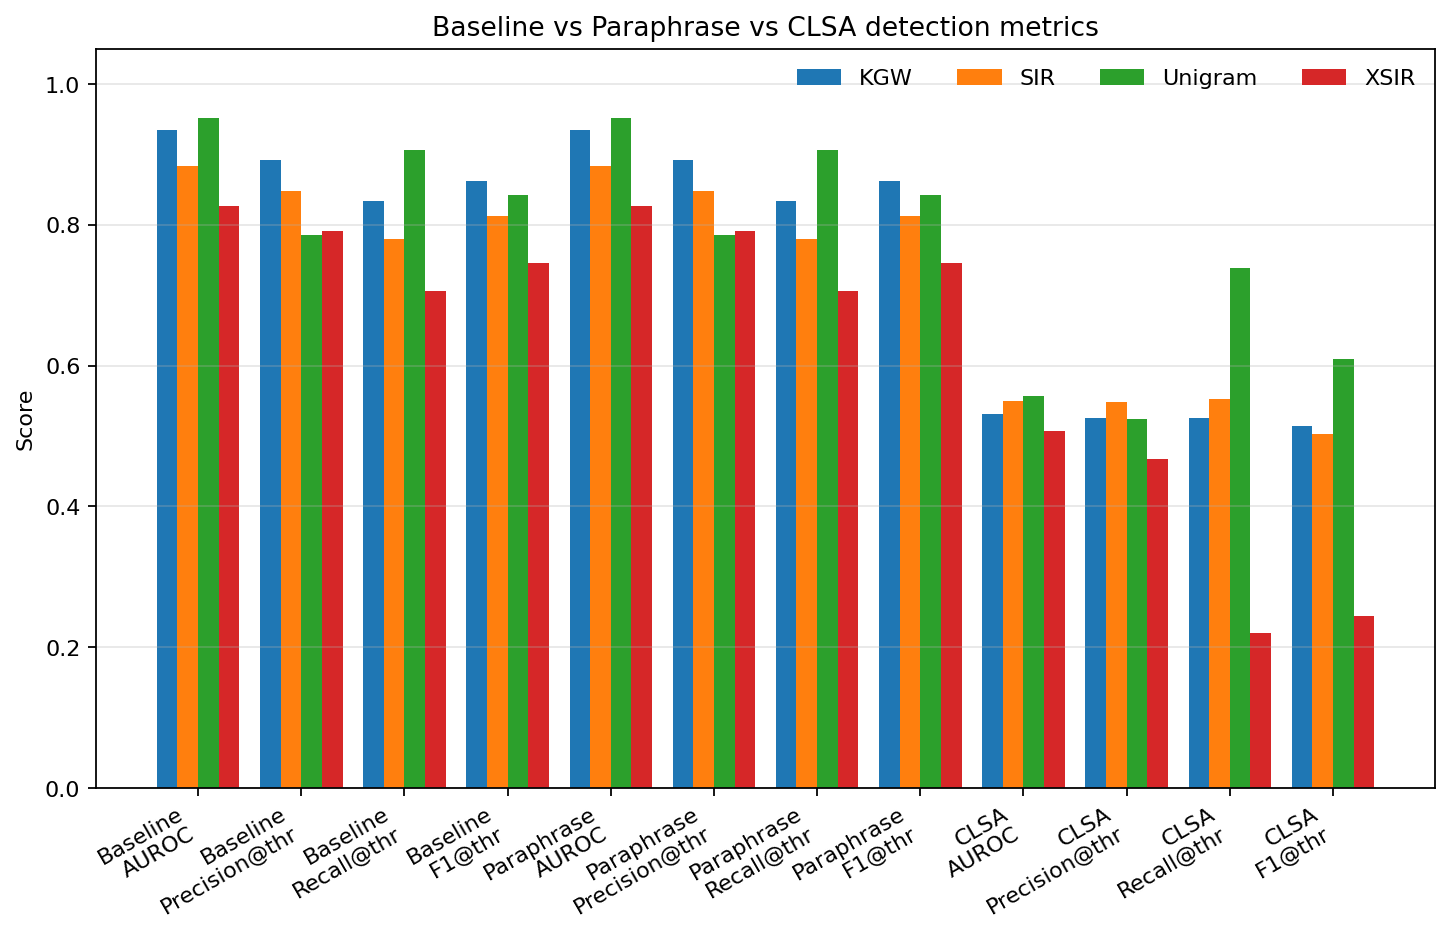
\includegraphics[width=\linewidth]{summary_metrics_bars.png}
\caption{\textbf{Summary metrics across detectors and languages.} Bars aggregate AUROC, AUPRC, Accuracy@thr, F1@thr, EER, and TPR@1\% FPR for baselines vs. CLSA. CLSA consistently drives AUROC toward chance (lower effective separability), increases EER, and collapses TPR@1\% FPR toward zero while keeping utility high.}
\label{fig:summary-bars}
\end{figure}

\textbf{Headline finding.}
Across KGW, SIR, XSIR, and Unigram, CLSA pushes detectors toward chance on all five languages with short, readable outputs. In Table~\ref{tab:auroc}, AUROCs under CLSA hover near 0.5 for XSIR on Amharic ($\approx$0.49), Chinese ($\approx$0.54), and Spanish ($\approx$0.51), and remain low for KGW on Spanish ($\approx$0.58). Back-translation and paraphrasing often leave stronger residual signal (e.g., Unigram on Hindi $\approx$0.61 under back-translation vs. $\approx$0.42 under CLSA). Figure~\ref{fig:summary-bars} shows the same trend across other metrics: EER rises under CLSA, while TPR@1\% FPR is typically near zero, indicating detectors cannot operate at low false-positive rates.

\textbf{XSIR stress test (cross-lingual robustness).}
For \textbf{XSIR} watermarking—explicitly designed for cross-lingual robustness—the AUROC under \emph{paraphrasing the base text} is $0.827$; under \emph{CWRA} with \emph{Chinese} as the pivot it is $0.823$; and under our \emph{CLSA} it falls to $0.53$, demonstrating that even the most robust cross-lingual watermarking scheme succumbs to our attack.

\textbf{Cross-detector analysis.}
KGW and Unigram show dramatic degradation (AUROC drops from 0.97+ to 0.42-0.67), while SIR and XSIR fare slightly better but still experience substantial degradation (0.49-0.57 vs. 0.97+). Low-resource languages show more severe degradation than high-resource ones, suggesting CLSA effectiveness scales with MT/summarization quality.

\section{Analysis and Discussion}

\textbf{Why summarization enables effective removal.}
CLSA's effectiveness stems from three key mechanisms: (1) \textbf{Position elimination}: Summarization removes 75-85\% of original positions, directly eliminating seeded tokens that KGW-family detectors rely on; (2) \textbf{Vocabulary consolidation}: Abstractive summarization favors high-frequency, generic vocabulary over diverse synonyms that may have been seeded; (3) \textbf{Semantic neighborhood disruption}: Cross-lingual summarization can map semantically similar source contexts to dissimilar target contexts, breaking SIR/XSIR clustering assumptions.

\textbf{Comparison with existing attacks.}
CLSA consistently outperforms alternatives: vs. paraphrasing (AUROC 0.42-0.67 vs. 0.65-0.82), vs. CWRA (0.42-0.67 vs. 0.46-0.82), and vs. back-translation (0.42-0.67 vs. 0.43-0.65), while providing practical length reduction benefits.

\textbf{Potential defenses.}
Defense directions include length-aware detection, multi-modal watermarking combining statistical and cryptographic approaches, and cross-lingual ensemble detection. However, these face fundamental limitations: length restrictions conflict with legitimate use cases, cryptographic approaches require infrastructure changes, and the semantic bottleneck imposed by cross-lingual summarization may be unavoidable without restricting NLP applications.

\section{Limitations}

Our evaluation has several key limitations: (1) \textbf{Scale}: Five languages and four detectors with 300 samples per language—results may vary across language families and document lengths; (2) \textbf{Quality metrics}: We rely on length ratios and qualitative assessment rather than comprehensive automatic metrics like ROUGE or human evaluation; (3) \textbf{Model dependence}: Results depend on specific models (M2M100, mT5/XLSum) and may not generalize to other architectures; (4) \textbf{Attack optimization}: We use straightforward implementations without adversarial optimization techniques.

\section{Broader Impact}

\textbf{Positive impacts:} This research advances understanding of watermark robustness and enables development of better defenses by identifying concrete failure modes. It highlights the importance of multi-modal approaches to AI accountability beyond statistical watermarks.

\textbf{Negative impacts:} The techniques could be misused for academic misconduct, disinformation, or circumventing AI safety measures. The simplicity of our approach—requiring only public models—lowers barriers for malicious actors.

\textbf{Mitigation:} We emphasize responsible disclosure, focus on defensive insights rather than attack optimization, and support policy implications that watermark-only approaches may be insufficient for high-stakes applications, requiring multi-modal verification strategies.

\section{Conclusion}

CLSA represents a simple yet effective watermark removal attack that exploits the fundamental tension between cross-lingual processing and distributional watermark detection. By forcing watermarked text through translation and summarization—operations that are increasingly common in real-world NLP pipelines—CLSA systematically erases statistical traces while preserving semantic content.

Our comprehensive evaluation across four watermarking schemes and five languages demonstrates that this attack consistently drives detection toward chance performance, often outperforming existing approaches while producing shorter, more readable outputs. These findings have immediate implications for watermark deployment and highlight fundamental limitations of purely distributional approaches to AI content verification.

The results call for a fundamental reconsideration of watermarking strategies in multilingual contexts. Future work should focus on developing watermarks that maintain stronger invariants across linguistic and compression boundaries, while also exploring hybrid approaches that combine statistical watermarks with cryptographic verification or model attestation.

More broadly, CLSA illustrates the challenges of securing AI systems in increasingly multilingual and multimodal environments. As language technologies become more sophisticated and accessible, adversarial techniques will inevitably evolve to exploit new vulnerabilities. Effective AI accountability will require adaptive strategies that anticipate and counter these developments through technical innovation, policy frameworks, and social norms.

The race between watermarking defenders and adversaries is far from over—but our findings suggest that current distributional approaches alone may be insufficient for high-stakes applications where security cannot be compromised by routine language processing operations.

\bibliographystyle{plainnat}
\bibliography{refs}

\appendix

\section{Detailed Results}

\begin{figure}[h]
\centering
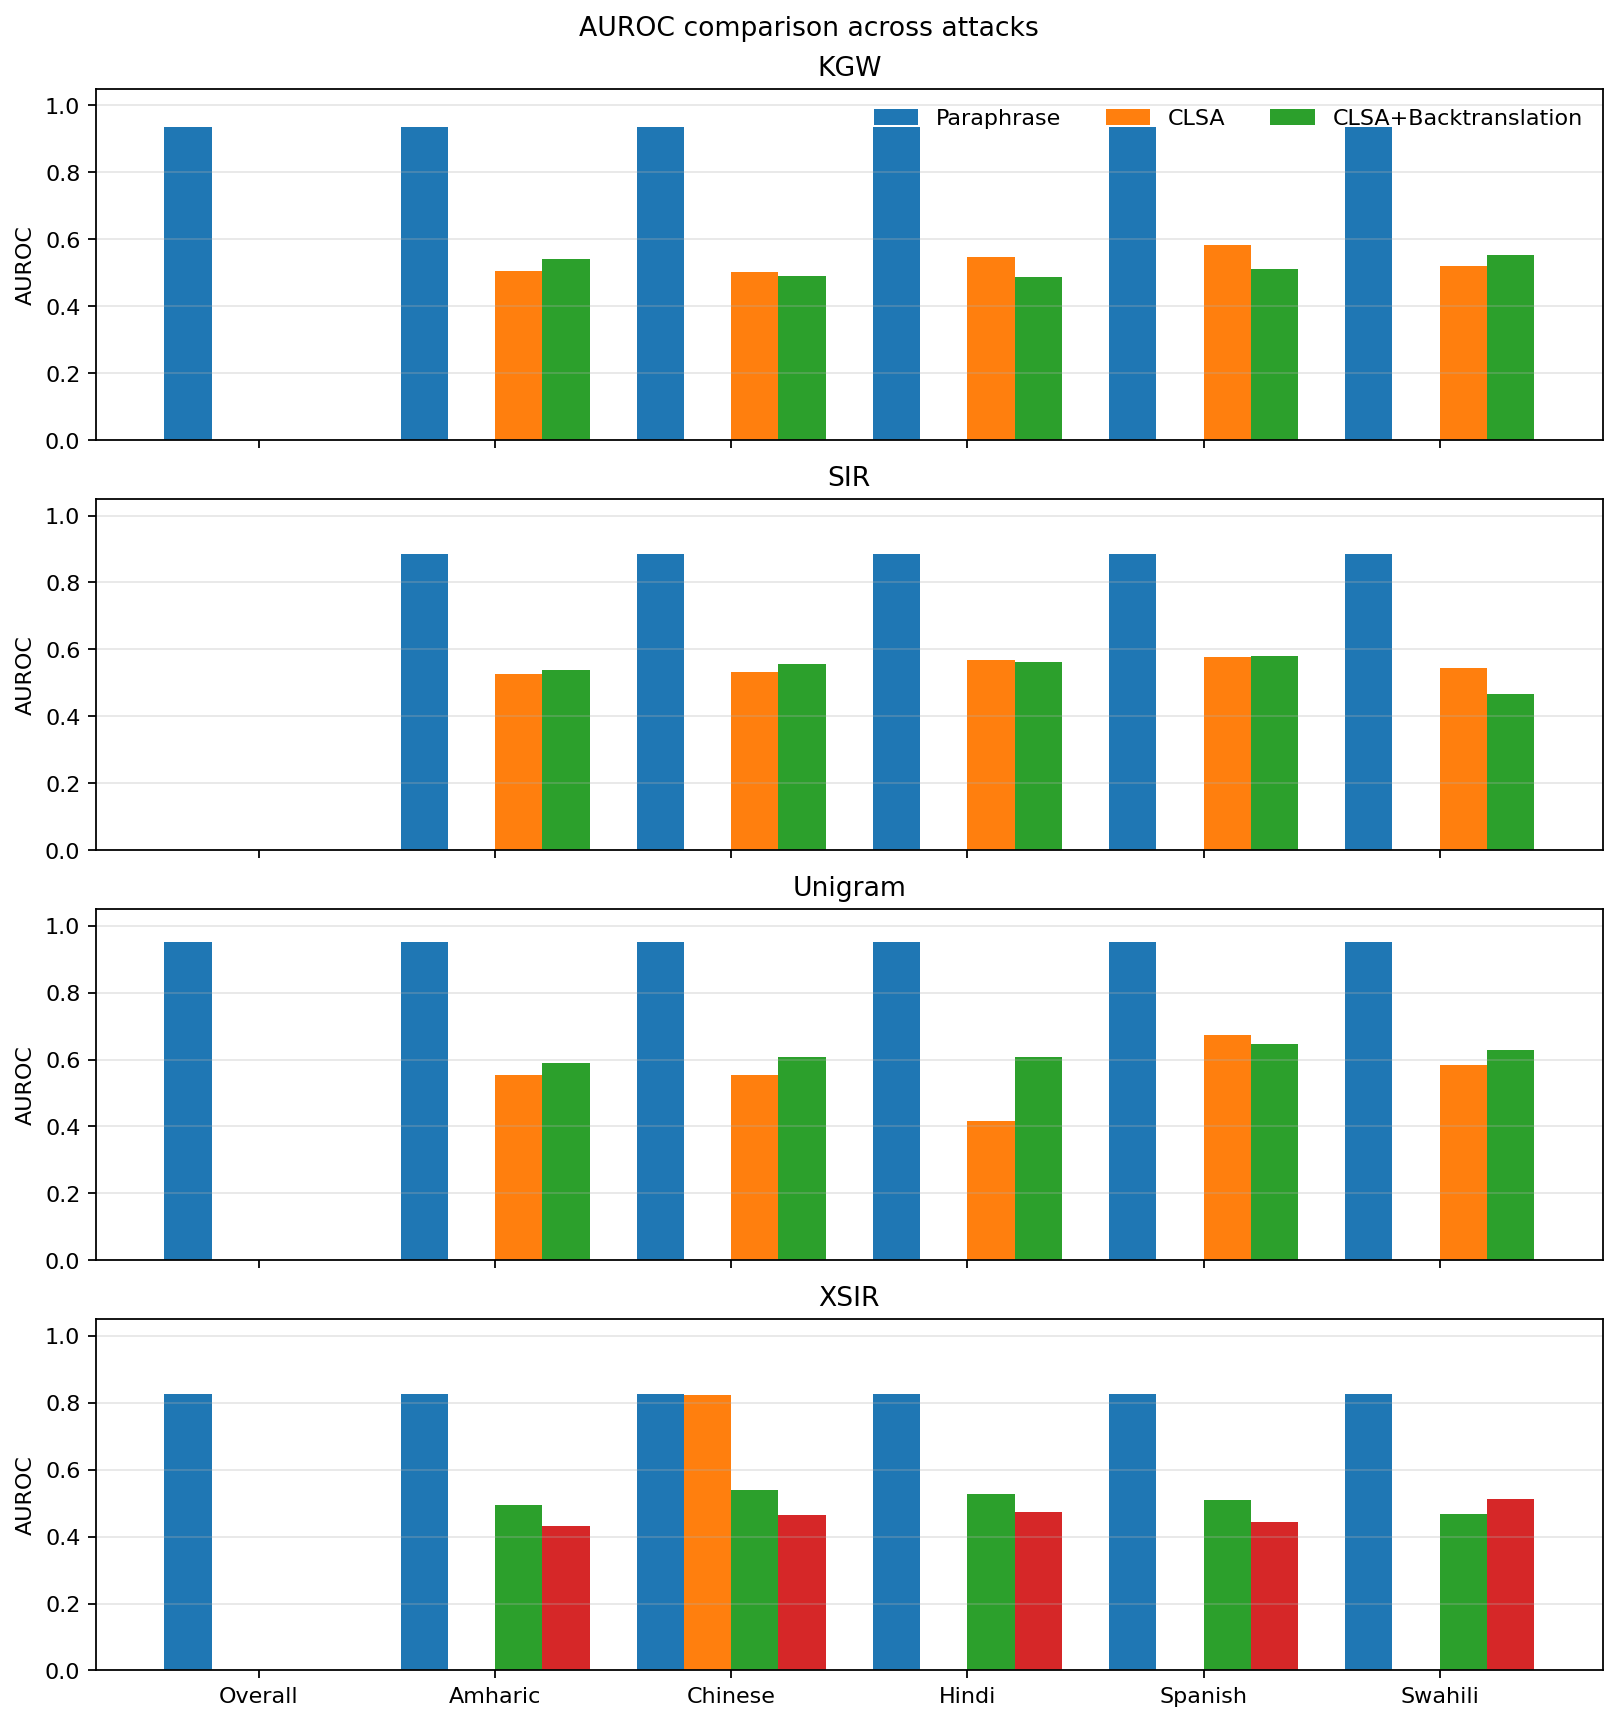
\includegraphics[width=\linewidth]{auroc_bars.png}
\caption{AUROC by detector and language. CLSA consistently trends toward chance performance across all evaluated combinations.}
\end{figure}

\begin{figure}[h]
\centering
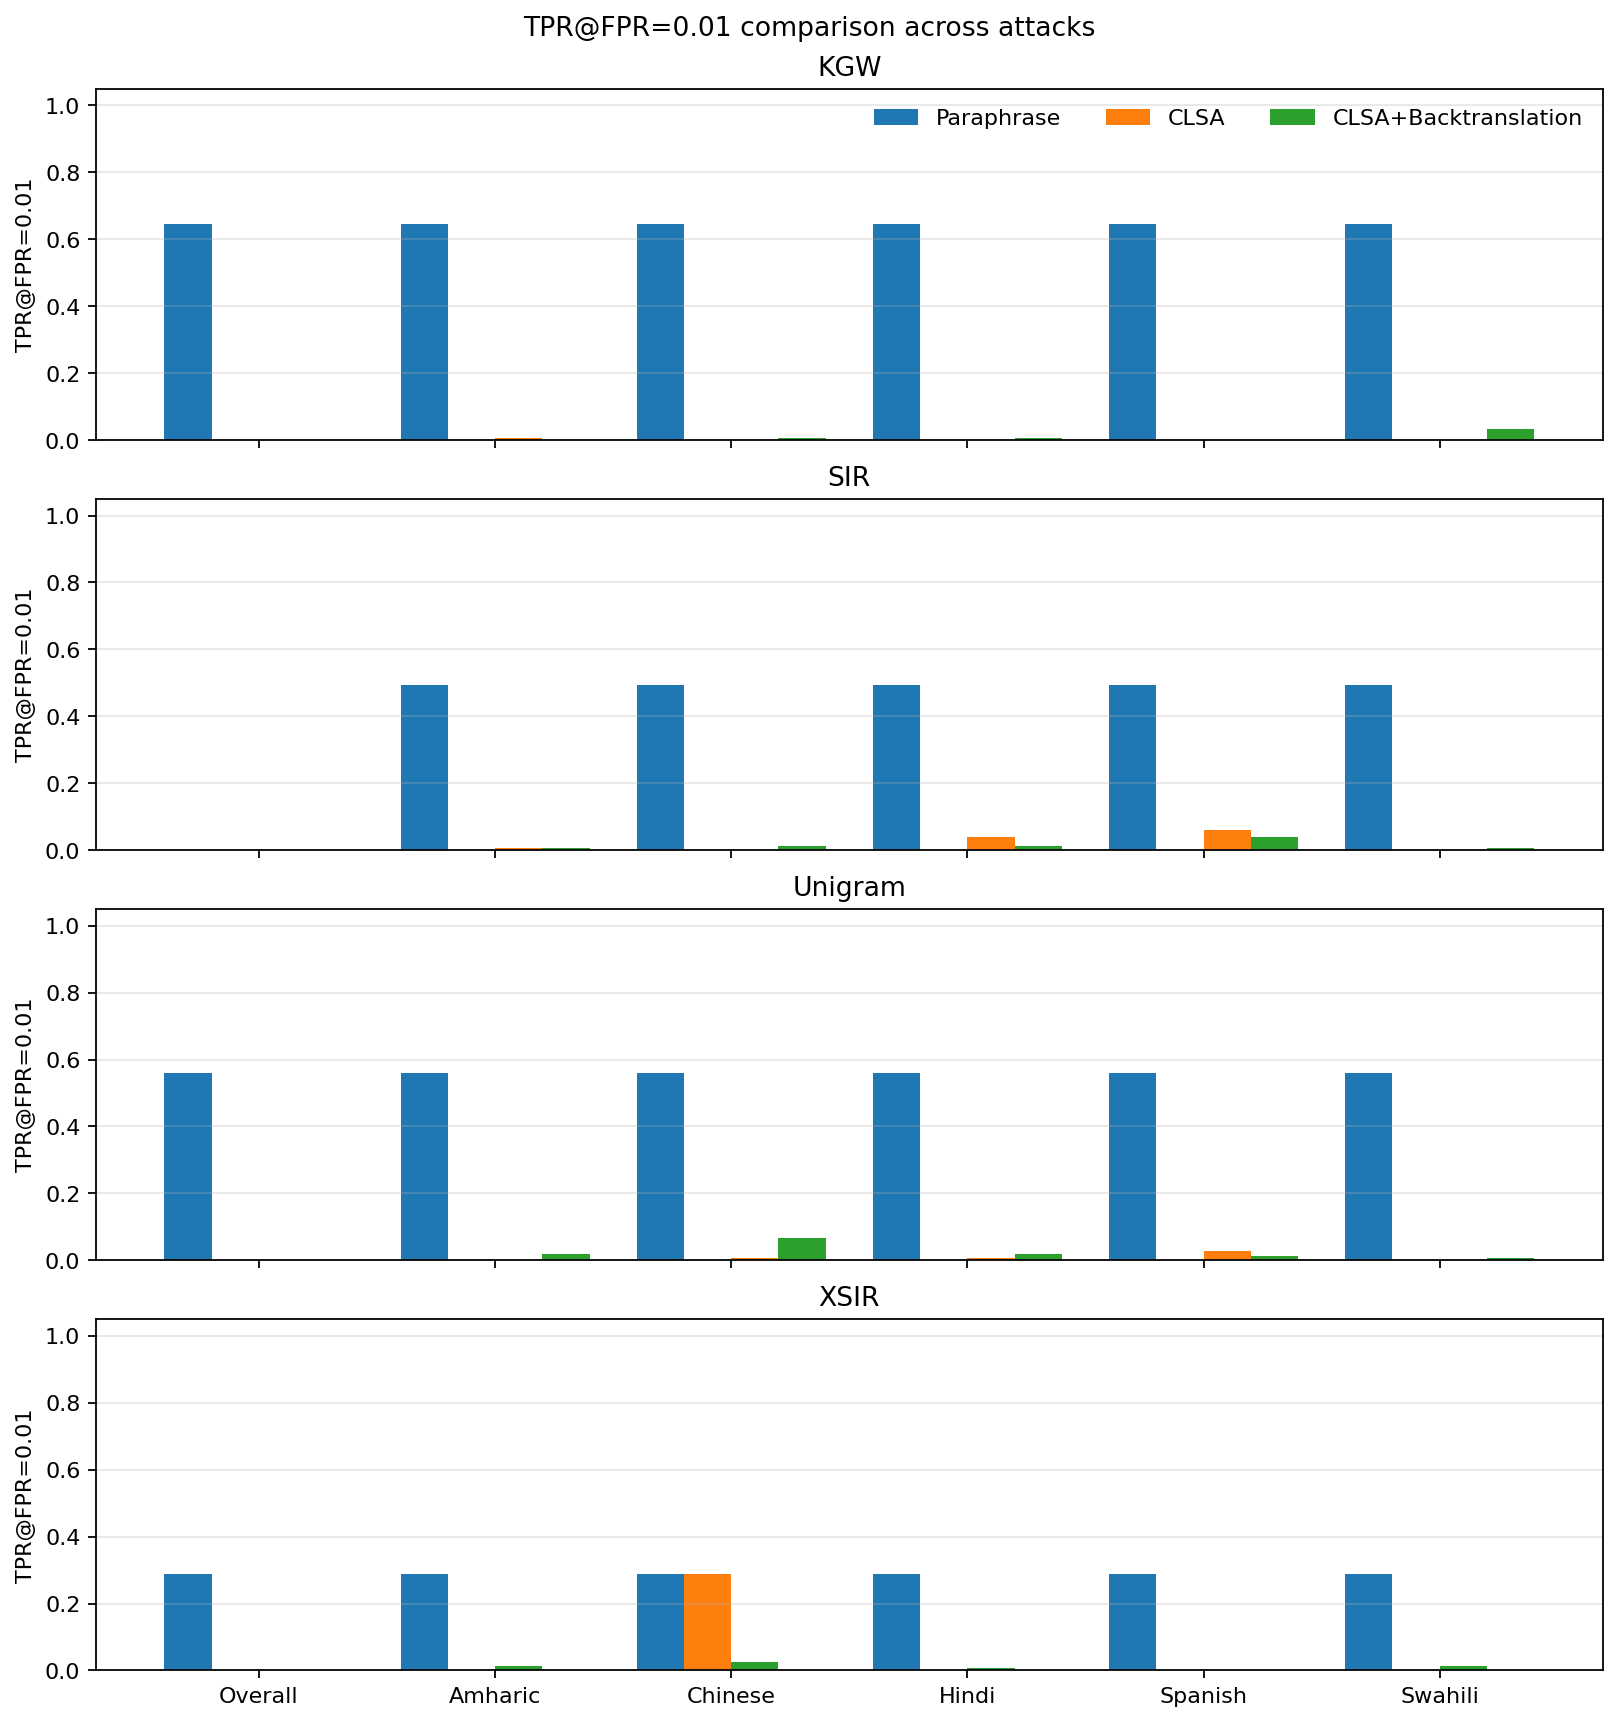
\includegraphics[width=\linewidth]{tpr_fpr_0_01_bars.png}
\caption{TPR at 1\% FPR: CLSA collapses true-positive rates at stringent false-positive operating points, indicating practical detection failure.}
\end{figure}

\begin{figure}[h]
\centering
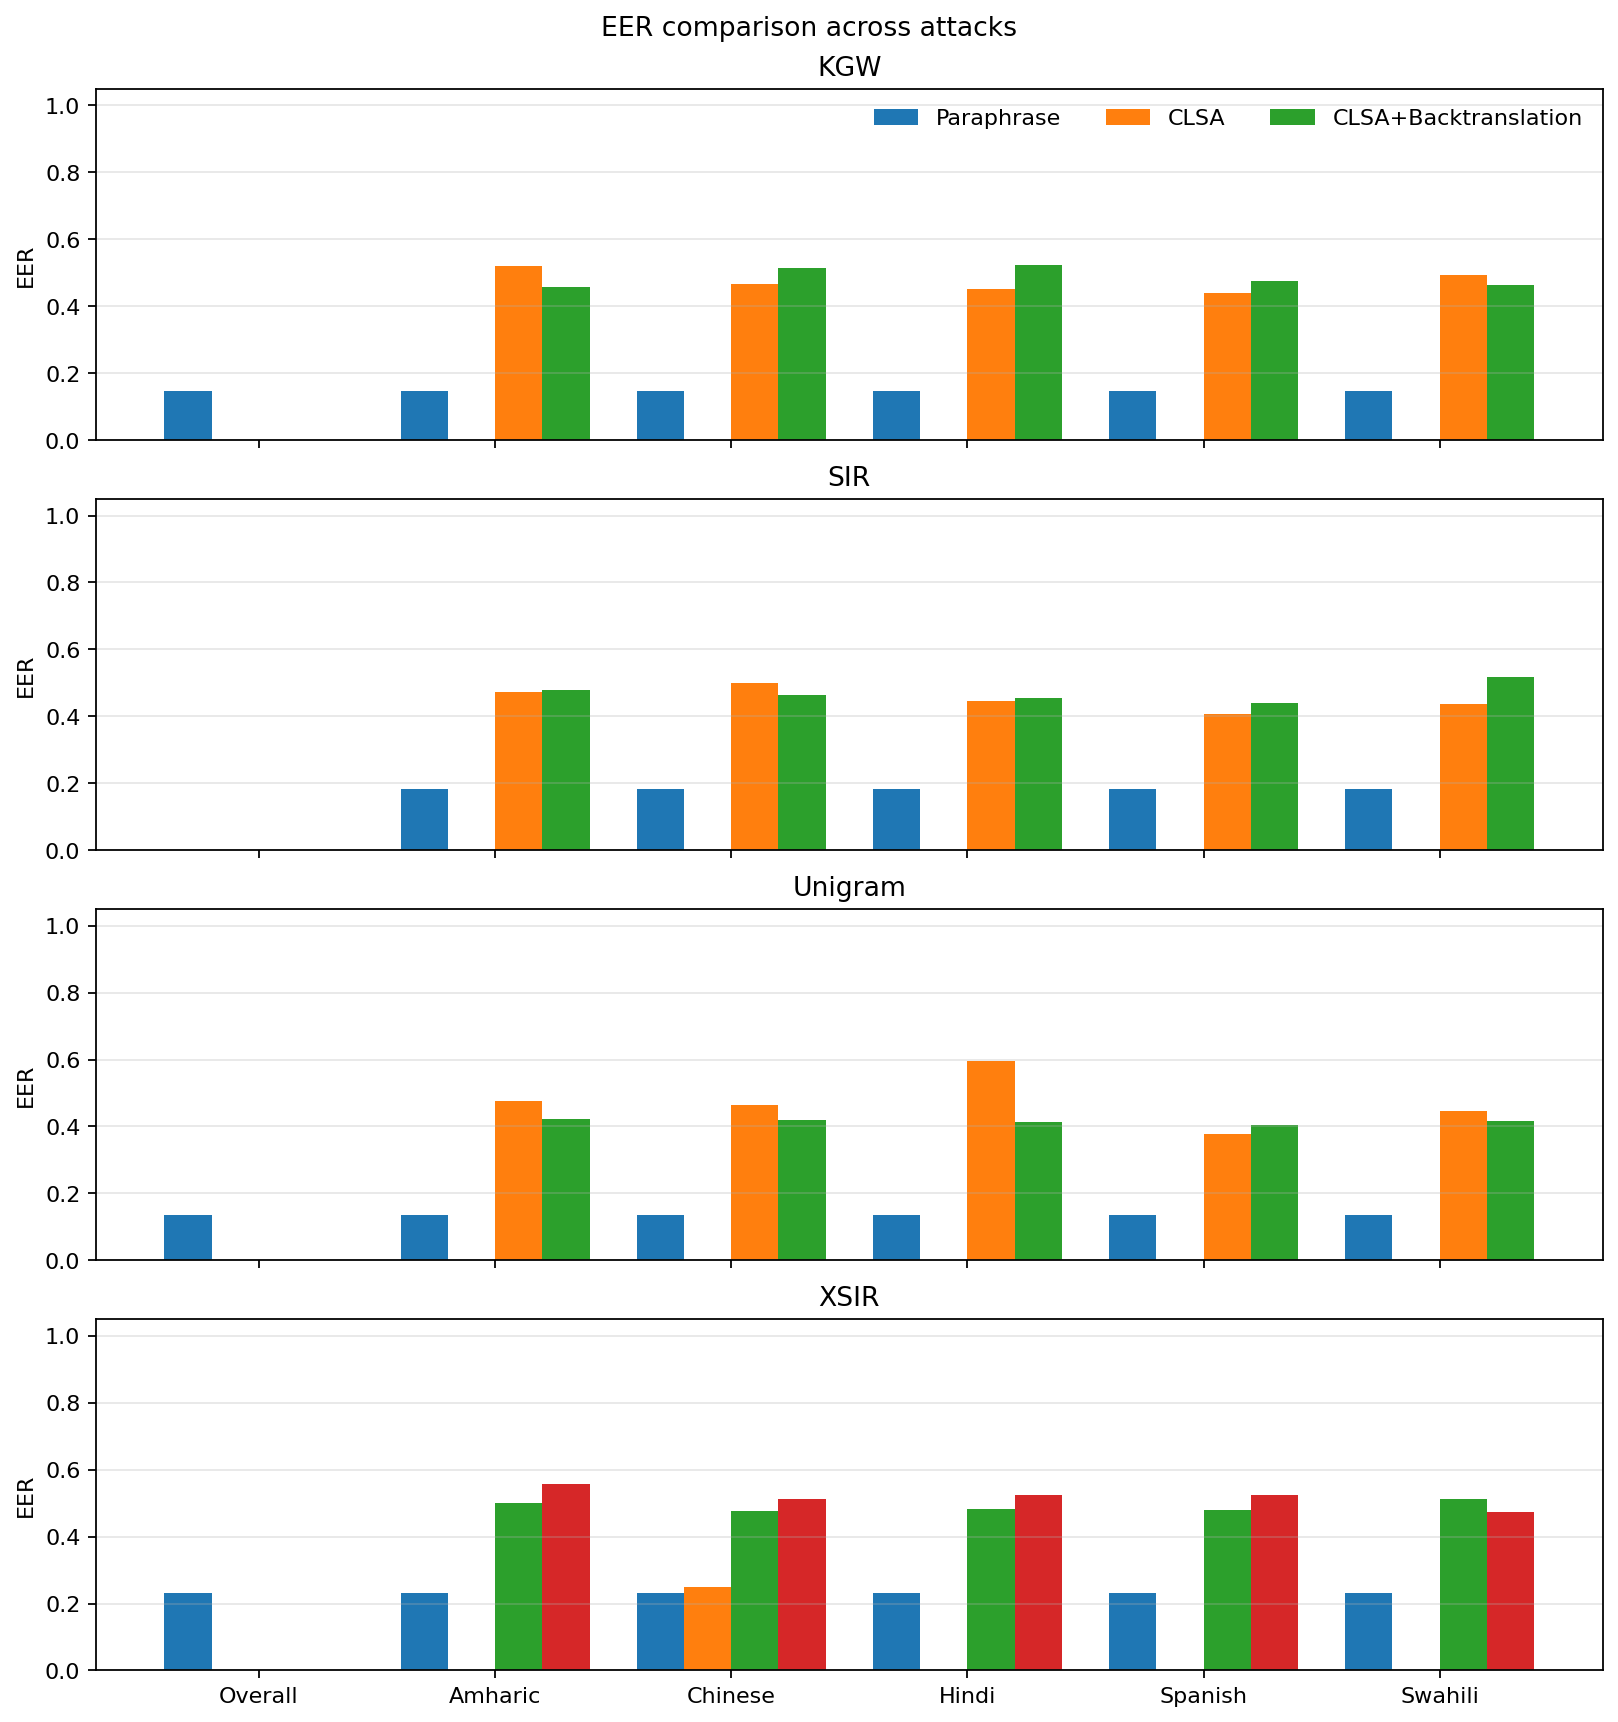
\includegraphics[width=\linewidth]{eer_bars.png}
\caption{Equal Error Rate (EER): higher values under CLSA indicate reduced separability between watermarked and non-watermarked content.}
\end{figure}

\end{document}